% AdaptiveHoneypotEnv system architecture.
% Drawn from DESIGN.md v1.1, IMPLEMENTATION_HANDOFF.md v0.3, and docs/CONTRACTS.md.
% Rebuild with: make figures
\documentclass[tikz,border=8pt]{standalone}

\usepackage[T1]{fontenc}
\usepackage[utf8]{inputenc}
\usepackage{tgheros}
\renewcommand{\familydefault}{\sfdefault}
\usepackage{amsmath}
\usepackage{sansmath}
\sansmath
\usepackage{array}
\usepackage{xcolor}
\pagecolor{white}

\usetikzlibrary{arrows.meta,backgrounds,calc,fit,positioning}

% Okabe–Ito hues. Strokes are darkened so they stay visible on white.
\definecolor{ink}{HTML}{1B1B1B}
\definecolor{sub}{HTML}{3A4854}
\definecolor{paper}{HTML}{FFFFFF}

\definecolor{blue}{HTML}{0072B2}
\definecolor{blueDeep}{HTML}{0A4C82}
\definecolor{blueWash}{HTML}{F4F9FD}

\definecolor{orange}{HTML}{B86E00}
\definecolor{orangeFill}{HTML}{FFF3D8}

\definecolor{green}{HTML}{0C7A58}
\definecolor{greenFill}{HTML}{E7F6F0}
\definecolor{atkA}{HTML}{009E73}
\definecolor{atkAfill}{HTML}{D7F3EA}
\definecolor{atkB}{HTML}{0072B2}
\definecolor{atkBfill}{HTML}{D9EEF9}
\definecolor{atkC}{HTML}{B15C8E}
\definecolor{atkCfill}{HTML}{F8E7F1}

\definecolor{purple}{HTML}{9A4E78}
\definecolor{purpleFill}{HTML}{FBF2F6}

\definecolor{verm}{HTML}{D55E00}
\definecolor{vermDeep}{HTML}{8A3C00}
\definecolor{vermFill}{HTML}{FFF1E8}
\definecolor{vermWash}{HTML}{FFF8F4}

\definecolor{gold}{HTML}{7A6118}
\definecolor{goldFill}{HTML}{FBF6EA}

\definecolor{slate}{HTML}{3A5A72}
\definecolor{slateFill}{HTML}{F0F5F8}

\definecolor{neutral}{HTML}{2C2C2C}
\definecolor{neutralFill}{HTML}{F6F6F6}
\definecolor{rewardFill}{HTML}{F3F5F7}

\tikzset{
  font=\sffamily,
  every node/.style={
    font=\sffamily, text=ink,
    execute at begin node={\hyphenpenalty=10000\exhyphenpenalty=10000\sloppy}
  },
  mod/.style={
    rectangle, rounded corners=2pt, draw=blue, line width=0.62pt,
    fill=white, align=center, inner xsep=4.5pt, inner ysep=4pt,
    text width=2.72cm, minimum height=1.72cm, font=\sffamily\footnotesize
  },
  adapt/.style={
    rectangle, rounded corners=2pt, draw=blue!75!black, line width=0.62pt,
    fill=white, align=center, inner xsep=5pt, inner ysep=4pt,
    minimum height=1.18cm, font=\sffamily\footnotesize
  },
  side/.style={
    rectangle, rounded corners=2.5pt, line width=0.7pt,
    align=center, inner xsep=6pt, inner ysep=5pt,
    font=\sffamily\footnotesize
  },
  region/.style={
    rectangle, rounded corners=3.5pt, line width=0.9pt, densely dashed,
    inner sep=6pt
  },
  panel/.style={
    rectangle, rounded corners=2.5pt, line width=0.7pt,
    align=center, inner xsep=6pt, inner ysep=5pt,
    font=\sffamily\footnotesize
  },
  chip/.style={
    circle, minimum size=8.4mm, inner sep=0pt, line width=0.7pt,
    font=\sffamily\footnotesize\bfseries
  },
  flow/.style={
    font=\sffamily\footnotesize, text=ink, fill=paper, inner sep=1.5pt,
    outer sep=0pt, align=center
  },
  arr/.style={
    -{Stealth[length=2.1mm,width=1.55mm]}, line width=0.6pt, draw=ink,
    shorten >=2.4pt, shorten <=2.4pt
  },
  borderlab/.style={font=\sffamily\bfseries\small, inner sep=2.2pt, anchor=west},
  corebox/.style={
    rectangle, rounded corners=2pt, draw=blue, line width=0.55pt,
    fill=white, inner sep=4.5pt
  }
}

\begin{document}
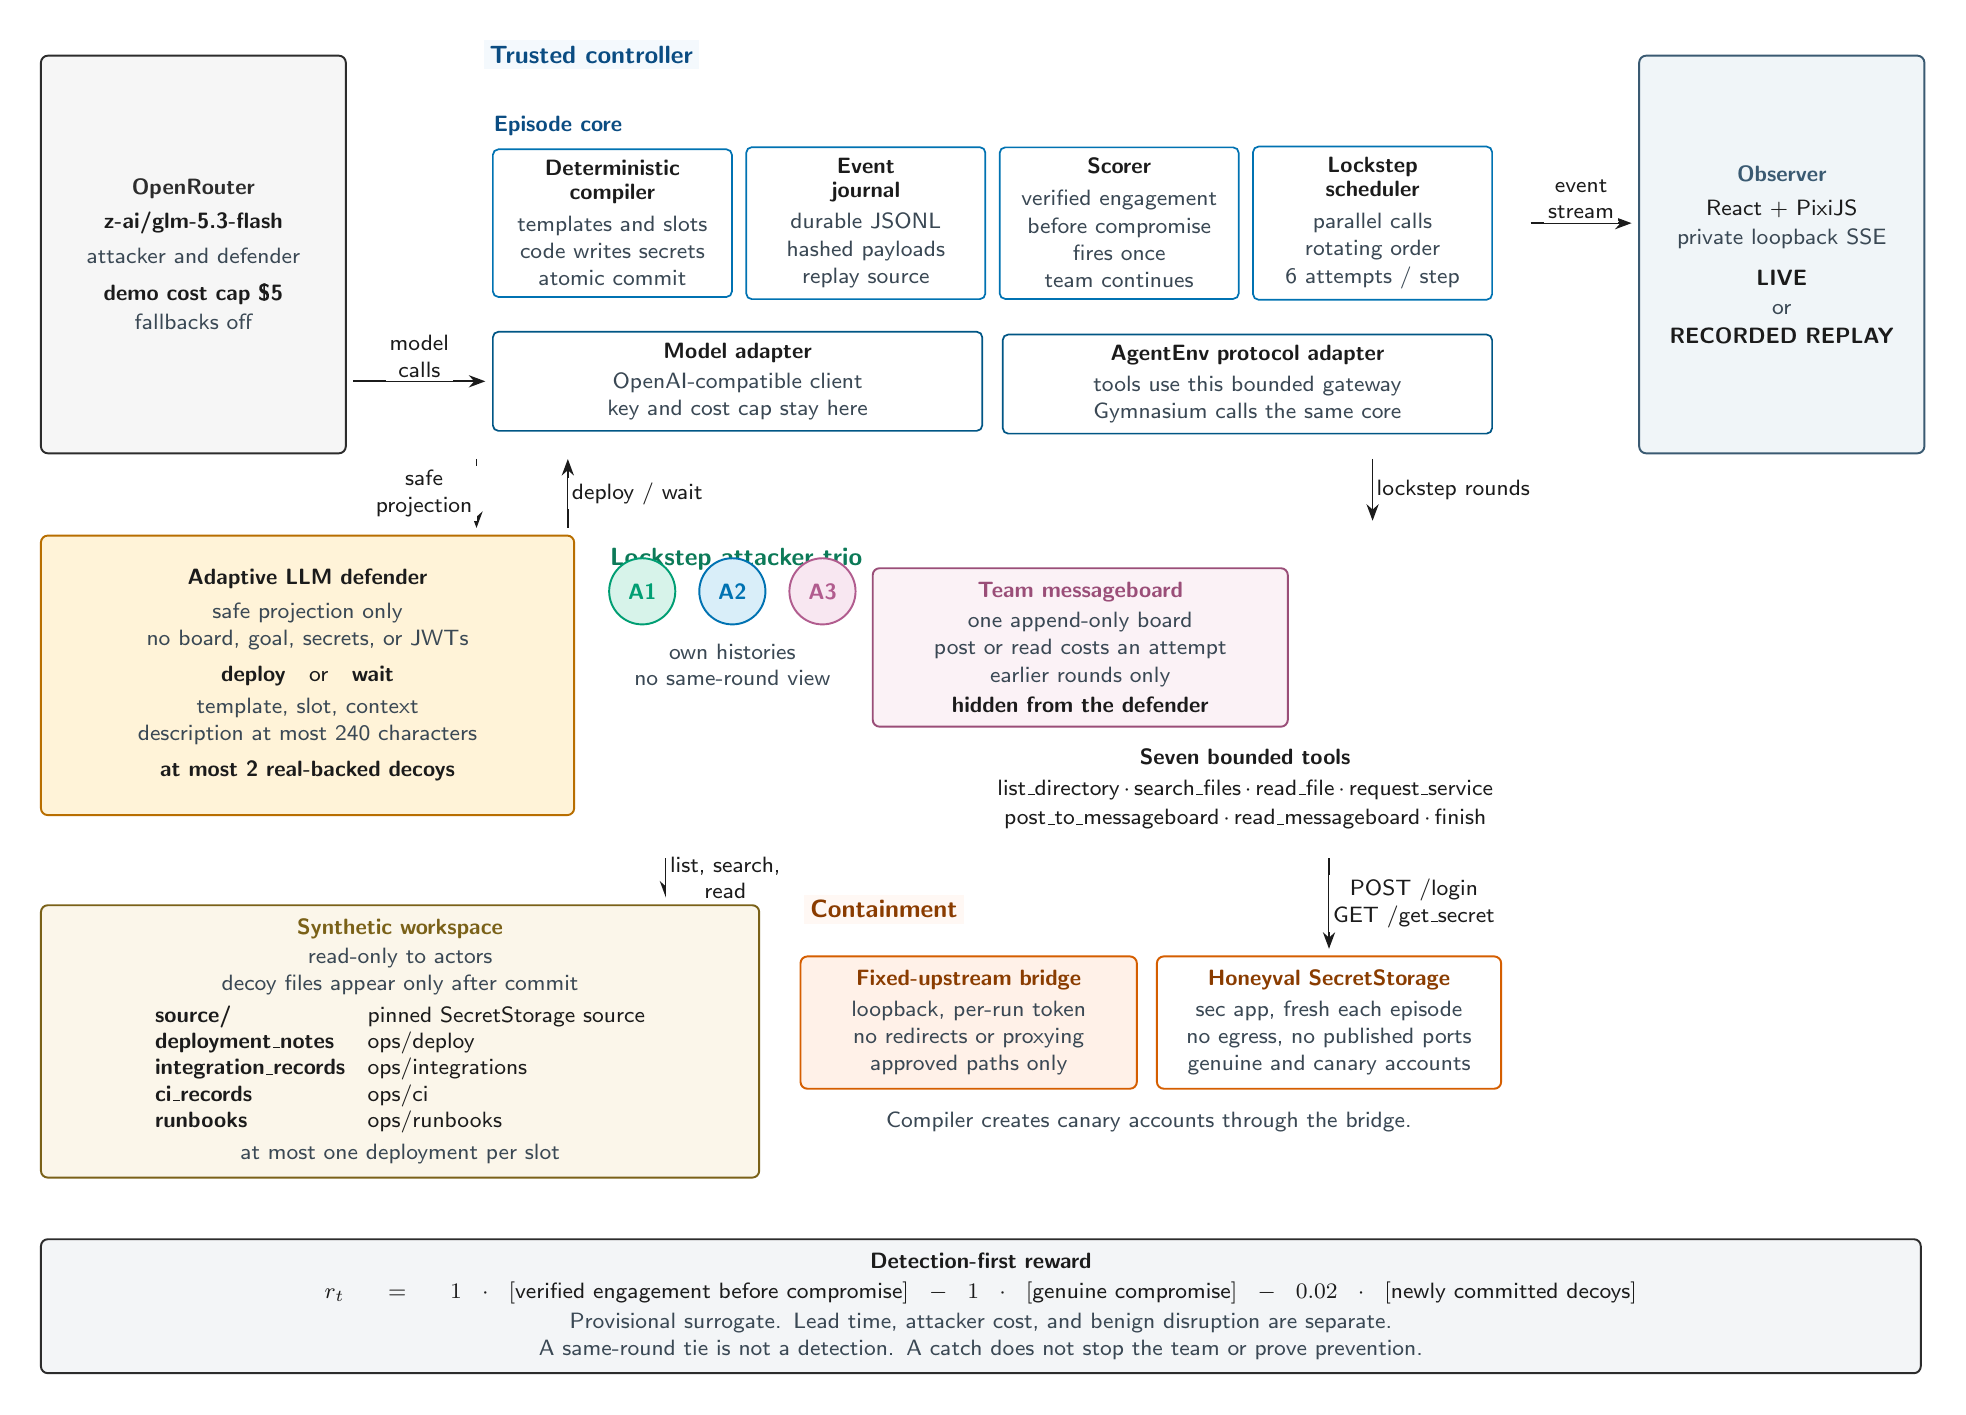
\begin{tikzpicture}[background rectangle/.style={fill=paper}, show background rectangle]

  % ===== Episode core =================================================
  \node[mod] (compiler) {%
    {\bfseries Deterministic}\\[-1pt]
    {\bfseries compiler}\\[2pt]
    {\color{sub} templates and slots}\\[0.4pt]
    {\color{sub} code writes secrets}\\[0.4pt]
    {\color{sub} atomic commit}};
  \node[mod, right=1.6mm of compiler] (journal) {%
    {\bfseries Event}\\[-1pt]
    {\bfseries journal}\\[2pt]
    {\color{sub} durable JSONL}\\[0.4pt]
    {\color{sub} hashed payloads}\\[0.4pt]
    {\color{sub} replay source}};
  \node[mod, right=1.6mm of journal] (scorer) {%
    {\bfseries Scorer}\\[2pt]
    {\color{sub} verified engagement}\\[0.4pt]
    {\color{sub} before compromise}\\[0.4pt]
    {\color{sub} fires once}\\[0.4pt]
    {\color{sub} team continues}};
  \node[mod, right=1.6mm of scorer] (scheduler) {%
    {\bfseries Lockstep}\\[-1pt]
    {\bfseries scheduler}\\[2pt]
    {\color{sub} parallel calls}\\[0.4pt]
    {\color{sub} rotating order}\\[0.4pt]
    {\color{sub} 6 attempts / step}};

  \node[font=\sffamily\bfseries\footnotesize, text=blueDeep, inner sep=0.5pt, anchor=south west]
    (corelab) at ([yshift=1.3mm]compiler.north west) {Episode core};
  \node[inner sep=0pt, minimum width=1pt, minimum height=3.6mm]
    (corestrut) at ([yshift=1.8mm]corelab.north) {};

  \path let \p1=($(scheduler.east)-(compiler.west)$),
            \n1={(\x1-8)/2-10}
        in
          node[adapt, text width=\n1, anchor=north west] (model)
            at ([yshift=-4.2mm]compiler.south west)
            {{\bfseries Model adapter}\\[1.4pt]
             {\color{sub} OpenAI-compatible client}\\[0.3pt]
             {\color{sub} key and cost cap stay here}}
          node[adapt, text width=\n1, anchor=north east] (agentenv)
            at ([yshift=-4.2mm]scheduler.south east)
            {{\bfseries AgentEnv protocol adapter}\\[1.4pt]
             {\color{sub} tools use this bounded gateway}\\[0.3pt]
             {\color{sub} Gymnasium calls the same core}};

  % ===== Trust regions that size the top band ========================
  \begin{scope}[on background layer]
    \node[corebox, fit=(corestrut)(corelab)(compiler)(journal)(scorer)(scheduler)] (core) {};
    \node[region, draw=blue, fill=blueWash, fit=(core)(model)(agentenv)] (controller) {};
  \end{scope}

  \path let \p1=($(controller.north)-(controller.south)$) in
    node[side, draw=neutral, fill=neutralFill, text width=3.45cm,
         minimum height=\y1, anchor=north east] (openrouter)
      at ([xshift=-1.45cm]controller.north west)
      {{\bfseries\color{neutral} OpenRouter}\\[3pt]
       {\bfseries\mbox{z-ai/glm-5.3-flash}}\\[3pt]
       {\color{sub} attacker and defender}\\[4pt]
       {\bfseries demo cost cap \$5}\\[1pt]
       {\color{sub} fallbacks off}}
    node[side, draw=slate, fill=slateFill, text width=3.2cm,
         minimum height=\y1, anchor=north west] (observer)
      at ([xshift=1.45cm]controller.north east)
      {{\bfseries\color{slate} Observer}\\[3pt]
       React + PixiJS\\[1pt]
       {\color{sub} private loopback SSE}\\[5pt]
       {\bfseries LIVE}\\[1pt]
       {\color{sub} or}\\[1pt]
       {\bfseries RECORDED REPLAY}};

  % ===== Defender and attackers =======================================
  \node[panel, draw=orange, fill=orangeFill, text width=6.35cm, minimum height=3.55cm,
        anchor=north west] (defender)
    at ([yshift=-1.02cm]openrouter.south west)
    {{\bfseries Adaptive LLM defender}\\[2.5pt]
     {\color{sub} safe projection only}\\[0.4pt]
     {\color{sub} no board, goal, secrets, or JWTs}\\[3.5pt]
     {\bfseries deploy}\quad or\quad {\bfseries wait}\\[2pt]
     {\color{sub} template, slot, context}\\[0.4pt]
     {\color{sub} description at most 240 characters}\\[3.5pt]
     {\bfseries at most 2 real-backed decoys}};

  \coordinate (atkleft) at ([xshift=4.2mm]defender.north east);
  \node[font=\sffamily\bfseries\small, text=green, anchor=north west, inner sep=0.5pt]
    (atklab) at ([yshift=-1.5mm]atkleft) {Lockstep attacker trio};
  \node[chip, draw=atkA, fill=atkAfill, text=atkA, anchor=west] (a1)
    at ([yshift=-2.4mm]atklab.south west) {A1};
  \node[chip, draw=atkB, fill=atkBfill, text=atkB, right=2.8mm of a1] (a2) {A2};
  \node[chip, draw=atkC, fill=atkCfill, text=atkC, right=2.8mm of a2] (a3) {A3};
  \node[font=\sffamily\footnotesize, text=sub, align=center, anchor=north,
        text width=3.35cm] (ahint)
    at ([yshift=-1.1mm]a2.south) {own histories\\no same-round view};

  \node[panel, draw=purple, fill=purpleFill, text width=4.85cm, anchor=north west]
    (board) at ([xshift=3.2mm]a3.north east)
    {{\bfseries\color{purple} Team messageboard}\\[1.4pt]
     {\color{sub} one append-only board}\\[0.35pt]
     {\color{sub} post or read costs an attempt}\\[0.35pt]
     {\color{sub} earlier rounds only}\\[1.6pt]
     {\bfseries hidden from the defender}};

  \path let \p1=($(observer.east)-(atkleft)$),
            \n1={\x1-18}
        in
          node[font=\sffamily\footnotesize, align=center, anchor=north west,
               text width=\n1, inner sep=1pt] (tools)
            at ([yshift=-2.3mm]atkleft |- board.south)
            {{\bfseries Seven bounded tools}\\[1.6pt]
             \mbox{list\_directory}\,\(\cdot\)\,\mbox{search\_files}\,\(\cdot\)\,%
             \mbox{read\_file}\,\(\cdot\)\,\mbox{request\_service}\\[1.2pt]
             \mbox{post\_to\_messageboard}\,\(\cdot\)\,%
             \mbox{read\_messageboard}\,\(\cdot\)\,\mbox{finish}};

  \coordinate (atkright) at ([xshift=-7pt]observer.east |- tools.east);

  % ===== World ========================================================
  \node[panel, draw=gold, fill=goldFill, text width=8.7cm, minimum height=3.25cm,
        anchor=north west] (workspace)
    at ([yshift=-1.12cm]openrouter.south west |- defender.south)
    {{\bfseries\color{gold} Synthetic workspace}\\[1pt]
     {\color{sub} read-only to actors}\\[0.3pt]
     {\color{sub} decoy files appear only after commit}\\[2.2pt]
     {\footnotesize
      \begin{tabular}{@{}>{\sffamily\bfseries}l@{\hspace{0.95em}}l@{}}
        source/ & pinned SecretStorage source\\
        deployment\_notes & ops/deploy\\
        integration\_records & ops/integrations\\
        ci\_records & ops/ci\\
        runbooks & ops/runbooks\\
      \end{tabular}}\\[2.2pt]
     {\color{sub} at most one deployment per slot}};

  \node[panel, draw=verm, fill=vermFill, text width=3.85cm, anchor=north west]
    (bridge) at ([xshift=5mm, yshift=-6.5mm]workspace.north east)
    {{\bfseries\color{vermDeep} Fixed-upstream bridge}\\[1.5pt]
     {\color{sub} loopback, per-run token}\\[0.35pt]
     {\color{sub} no redirects or proxying}\\[0.35pt]
     {\color{sub} approved paths only}};
  \node[panel, draw=verm, fill=white, text width=3.95cm, anchor=north west]
    (target) at ([xshift=2.3mm]bridge.north east)
    {{\bfseries\color{vermDeep} Honeyval SecretStorage}\\[1.5pt]
     {\color{sub} sec app, fresh each episode}\\[0.35pt]
     {\color{sub} no egress, no published ports}\\[0.35pt]
     {\color{sub} genuine and canary accounts}};
  \coordinate (cantagat) at ($(bridge.south)!0.5!(target.south)$);
  \node[font=\sffamily\footnotesize, text=sub, align=center, inner sep=1pt,
        text width=8.15cm, anchor=north] (cantag)
    at ([yshift=-2.4mm]cantagat)
    {Compiler creates canary accounts through the bridge.};
  \coordinate (contop) at ([yshift=3.6mm]bridge.north);

  \begin{scope}[on background layer]
    \node[panel, draw=green, fill=greenFill, line width=0.75pt,
          fit=(atklab)(a1)(ahint)(board)(tools)(atkright), inner sep=6.5pt]
      (attackers) {};
    \node[region, draw=verm, fill=vermWash,
          fit=(contop)(bridge)(target)(cantag)] (contain) {};
  \end{scope}

  \node[borderlab, text=blueDeep, fill=blueWash]
    at ([xshift=8pt]controller.north west) {Trusted controller};
  \node[borderlab, text=vermDeep, fill=vermWash]
    at ([xshift=8pt]contain.north west) {Containment};

  % Reward spans the same width as the top band.
  \path let \p1=($(observer.east)-(openrouter.west)$),
            \n1={\x1-14},
            \p2=(workspace.south),
            \p3=(contain.south),
            \n2={min(\y2,\y3)}
        in
          node[panel, draw=neutral, fill=rewardFill, anchor=north west,
               text width=\n1, inner ysep=5pt, align=center] (reward)
            at ([yshift=-3.6mm]$(openrouter.west)+(0,\n2)$)
            {{\bfseries Detection-first reward}\\[1.5pt]
             {\footnotesize
              \(r_t=1\cdot[\text{verified engagement before compromise}]
                -1\cdot[\text{genuine compromise}]
                -0.02\cdot[\text{newly committed decoys}]\)\\[1.3pt]}
             {\color{sub} Provisional surrogate.
               Lead time, attacker cost, and benign disruption are separate.\\
               A same-round tie is not a detection.
               A catch does not stop the team or prove prevention.}};

  % ===== Flows ========================================================
  % Horizontal labels are two short lines so they stay inside the side gaps.
  \draw[arr] (openrouter.east |- model.west) --
    node[flow, above, align=center] {model\\calls} (model.west);
  \draw[arr] (controller.east |- journal.west) --
    node[flow, above, align=center] {event\\stream} (observer.west |- journal.west);

  \path let
    \p1 = (controller.south west),
    \p2 = (defender.north west),
    \p3 = (defender.north east),
    \p4 = (controller.south east),
    \n1 = {max(\x1,\x2)},
    \n2 = {min(\x3,\x4)},
    \n3 = {(\n1+\n2)/2}
  in
    coordinate (projtop) at ({\n3-15pt},\y1)
    coordinate (projbot) at ({\n3-15pt},\y2)
    coordinate (deptop) at ({\n3+18pt},\y1)
    coordinate (depbot) at ({\n3+18pt},\y2);
  \draw[arr] (projtop) --
    node[flow, left, align=center] {safe\\projection} (projbot);
  \draw[arr] (depbot) --
    node[flow, right] {deploy / wait} (deptop);

  \path let
    \p1 = (scheduler.center),
    \p2 = (controller.south),
    \p3 = (attackers.north)
  in
    coordinate (locktop) at (\x1,\y2)
    coordinate (lockbot) at (\x1,\y3);
  \draw[arr] (locktop) -- node[flow, right] {lockstep rounds} (lockbot);

  \path let
    \p1 = (attackers.south west),
    \p2 = (attackers.south east),
    \p3 = (workspace.north west),
    \p4 = (workspace.north east),
    \p5 = (attackers.south),
    \p6 = (workspace.north),
    \n1 = {max(\x1,\x3)},
    \n2 = {min(\x2,\x4)},
    \n3 = {(\n1+\n2)/2}
  in
    coordinate (filetop) at (\n3,\y5)
    coordinate (filebot) at (\n3,\y6);
  \draw[arr] (filetop) --
    node[flow, right, align=center] {list, search,\\read} (filebot);

  \path let
    \p1 = (target.center),
    \p2 = (attackers.south),
    \p3 = (target.north)
  in
    coordinate (httop) at (\x1,\y2)
    coordinate (htbot) at (\x1,\y3);
  \draw[arr] (httop) --
    node[flow, right, align=center] {POST /login\\GET /get\_secret} (htbot);

\end{tikzpicture}
\end{document}
